%%%%%%%%%%%%%%%%%%%%%%%%%%%%%%%%%%%%%%%%%
% Beamer Presentation
% LaTeX Template
% Version 1.0 (10/11/12)
%
% This template has been downloaded from:
% http://www.LaTeXTemplates.com
%
% License:
% CC BY-NC-SA 3.0 (http://creativecommons.org/licenses/by-nc-sa/3.0/)
%
%%%%%%%%%%%%%%%%%%%%%%%%%%%%%%%%%%%%%%%%%

%----------------------------------------------------------------------------------------
%	PACKAGES AND THEMES
%----------------------------------------------------------------------------------------

\documentclass{beamer}

\mode<presentation> {

% The Beamer class comes with a number of default slide themes
% which change the colors and layouts of slides. Below this is a list
% of all the themes, uncomment each in turn to see what they look like.

%\usetheme{default}
%\usetheme{AnnArbor}
%\usetheme{Antibes}
%\usetheme{Bergen}
%\usetheme{Berkeley}
%\usetheme{Berlin}
%\usetheme{Boadilla}
%\usetheme{CambridgeUS}
%\usetheme{Copenhagen}
%\usetheme{Darmstadt}
%\usetheme{Dresden}
%\usetheme{Frankfurt}
%\usetheme{Goettingen}
%\usetheme{Hannover}
%\usetheme{Ilmenau}
%\usetheme{JuanLesPins}
%\usetheme{Luebeck}
%
\usetheme{Madrid}
%\usetheme{Malmoe}
%\usetheme{Marburg}
%\usetheme{Montpellier}
%\usetheme{PaloAlto}
%\usetheme{Pittsburgh}
%\usetheme{Rochester}
%\usetheme{Singapore}
%\usetheme{Szeged}
%\usetheme{Warsaw}

% As well as themes, the Beamer class has a number of color themes
% for any slide theme. Uncomment each of these in turn to see how it
% changes the colors of your current slide theme.

%\usecolortheme{albatross}
%\usecolortheme{beaver}
%\usecolortheme{beetle}
%\usecolortheme{crane}
%\usecolortheme{dolphin}
%\usecolortheme{dove}
%\usecolortheme{fly}
%\usecolortheme{lily}
%\usecolortheme{orchid}
%\usecolortheme{rose}
%
\usecolortheme{seagull}
%\usecolortheme{seahorse}
%\usecolortheme{whale}
%\usecolortheme{wolverine}

%\setbeamertemplate{footline} % To remove the footer line in all slides uncomment this line
%\setbeamertemplate{footline}[page number] % To replace the footer line in all slides with a simple slide count uncomment this line

%\setbeamertemplate{navigation symbols}{} % To remove the navigation symbols from the bottom of all slides uncomment this line
}

\usepackage{graphicx} % Allows including images
\usepackage{booktabs} % Allows the use of \toprule, \midrule and \bottomrule in tables


\usepackage[ final ]{pdfpages}
%----------------------------------------------------------------------------------------
%	TITLE PAGE
%----------------------------------------------------------------------------------------

\title[Software ontwerp: iteratie 1]{Software ontwerp: iteratie 1 (groep 8)} % The short title appears at the bottom of every slide, the full title is only on the title page

\author[Groep 8]{\\
		Andr\'e Jacobs \\
		Menno Keustermans\\
		Bruno Lannoo \\
		Thomas Marcelis} % Your name
\institute[KULeuven] % Your institution as it will appear on the bottom of every slide, may be shorthand to save space
{\\ % Your institution for the title page
\medskip
\textit{} % Your email address
}
\date{} % Date, can be changed to a custom date
\usepackage{graphicx}
\usepackage{caption}
\usepackage{subcaption}
\begin{document}

\begin{frame}
\titlepage % Print the title page as the first slide
\end{frame}


%----------------------------------------------------------------------------------------
%	PRESENTATION SLIDES
%----------------------------------------------------------------------------------------

%----------------------------------------------------------------------------------------
%	Packages overzicht:
%		In src zijn er 4 packages:
%		
%		Front-end : user interface
%					-> gebruikt exception, parser en taskmanager
%		Back-end : taskManager
%----------------------------------------------------------------------------------------

\begin{frame}
\frametitle {Packages: overzicht}
\begin{figure}
\centering
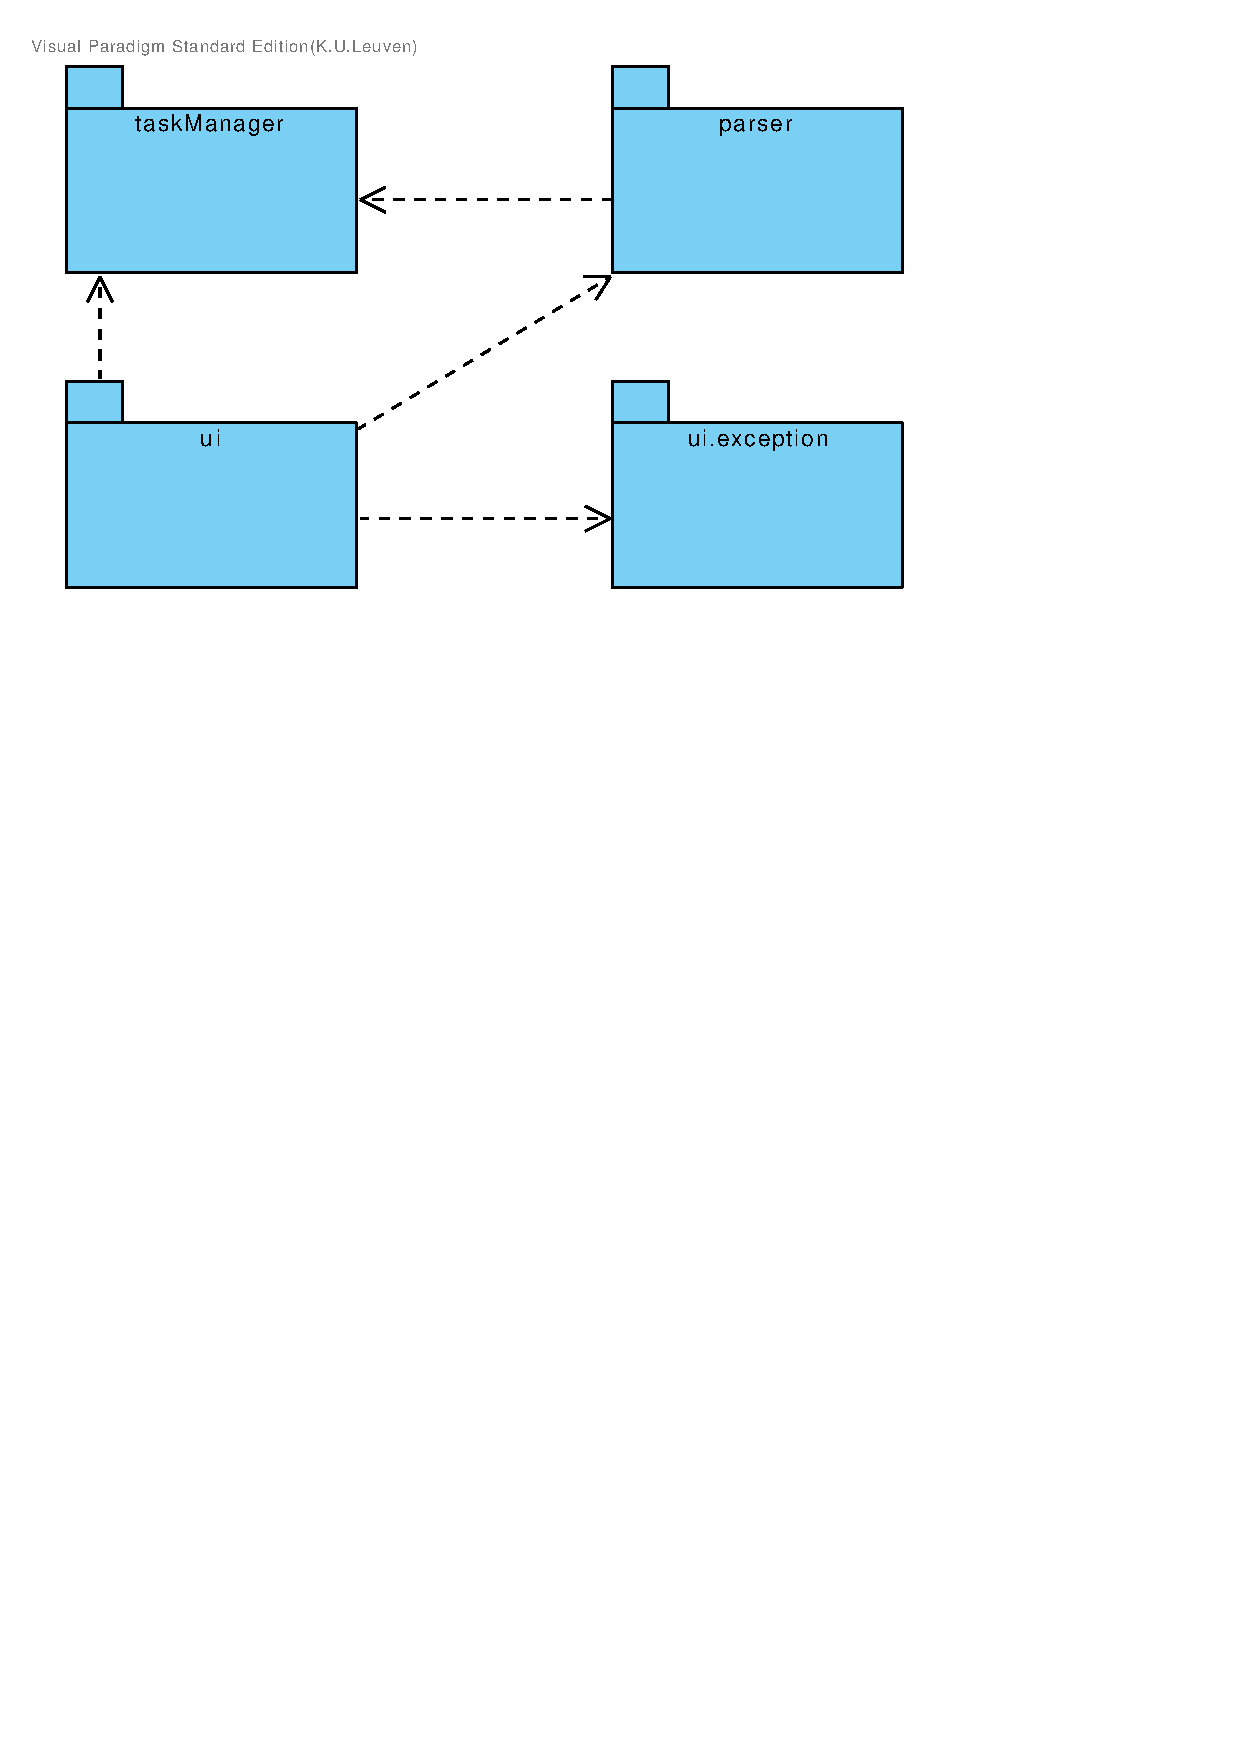
\includegraphics[width=1.3\textwidth]{figures/PackageDiagram.pdf}
\caption{Test}
\end{figure}
\end{frame}

%----------------------------------------------------------------------------------------
%	Class diagram overzicht: (back-end)
%		Project-controller heeft overzicht over alle projecten en bevat
%		de interne klok van het systeem
%
%		Project heeft overzicht van alle taken
%
%		Taken
%
%----------------------------------------------------------------------------------------

\begin{frame}
\frametitle {Class diagram: overzicht}
\begin{figure}
\centering
\begin{center}
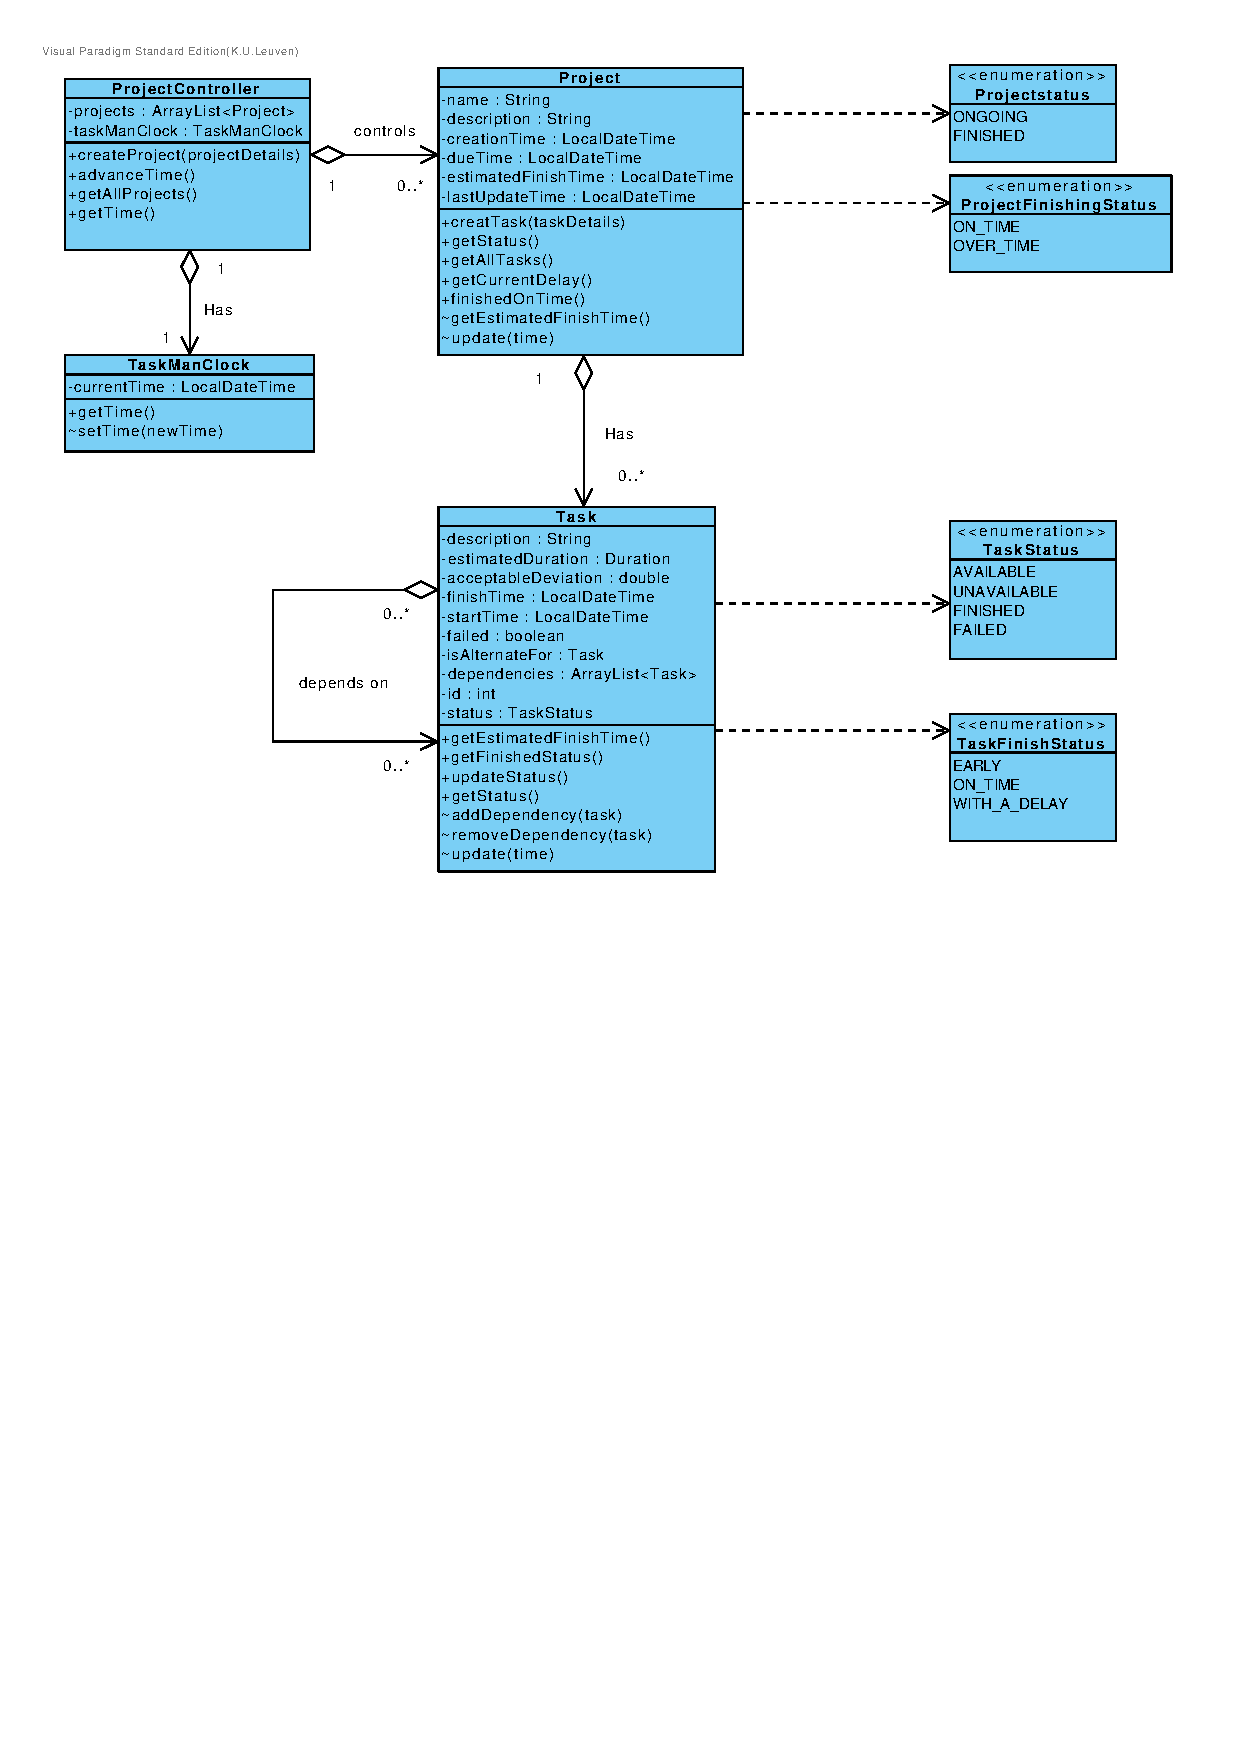
\includegraphics[width=0.92\textwidth]{figures/ClassDiagram.pdf}
\end{center}

\end{figure}
\end{frame}

%----------------------------------------------------------------------------------------
%	ProjectController (discussion GRASP)
%		Information expert
%			Verantwoordelijkheden:
%				- houdt lijst van projecten bij
%				- houdt ook de klok bij
%
%			Creator:
%				Verantwoordelijkheden: 
%				- Maakt elk project aan.
%	
%			Controller:
%				Aanspreekpunt voor alle informatie
%
%----------------------------------------------------------------------------------------

\begin{frame}
\frametitle {ProjectController: Grasp Patterns}
\begin{columns}
	\begin{column}{.45\paperwidth}
	\begin{itemize}
		\item Information expert:
			\begin{itemize}
				\item Kent alle projecten
				\item Kent de klok
			\end{itemize}
		\item Creator:
			\begin{itemize}
				\item Maakt de projecten aan
			\end{itemize}
		\item Controller:
			\begin{itemize}
				\item Aanspreekpunt voor alle UC
			\end{itemize}
	\end{itemize}
	\end{column}
	\begin{column}{.45\paperwidth}
		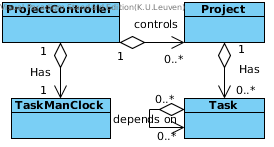
\includegraphics[width=0.4\paperwidth]{figures/MiniClassDiagram.png}
	\end{column}
\end{columns}
\end{frame}

%----------------------------------------------------------------------------------------
%	Testing
%		Unit testing: om corner cases te testen
%       Use Case testing: succes scenarios getest
%
%----------------------------------------------------------------------------------------

\begin{frame}
\frametitle {Testing}
\begin{itemize}
	\item Unit testing: om corner cases te testen
	\item Use Case testing: succes scenarios getest
\end{itemize}
\begin{columns}
	\begin{column}{.4\paperwidth}
		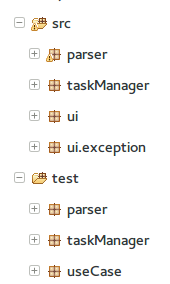
\includegraphics[width=0.2\paperwidth]{figures/Package_overview_eclipse.png}
	\end{column}
	\begin{column}{.4\paperwidth}
		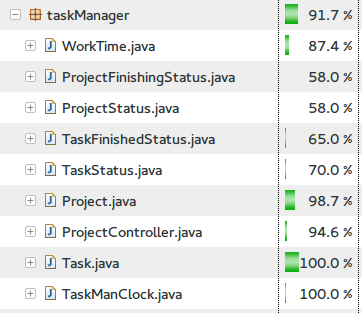
\includegraphics[width=0.35\paperwidth]{figures/coverage.png}
	\end{column}
\end{columns}
\end{frame}

\end{document} 
